This chapter provides an overview of the developed command-line tool for detecting the seven targeted SQL antipatterns, which employs the most effective prompting strategy identified based on the analysis that was described in Section~\ref{sec:experimentsQuantitative}. We discuss the tool's architectural design, internal workflow, and configuration options, as well as the coding process used to implement it.

The tool was developed with the assistance of OpenAI Codex \nobreakcite{openAiCodex2026GitHub}, using the GPT-5.4 \nobreakcite{gpt54} model, in a semi-autonomous agentic coding process. The development process was organised around iterative implementation tasks. For each task, we specified the intended behaviour, constraints, and expected outcome, after which the coding agent inspected the existing codebase, proposed or implemented the necessary changes, and ran relevant checks where applicable. Human supervision was retained throughout the process: generated changes were reviewed, requirements were clarified when necessary, and architectural decisions, evaluation requirements, and final acceptance of the implementation remained under human control. In this way, Codex was used primarily as an implementation assistant, while the design goals and validation criteria were defined by us.

\section{Architecture}

We implemented the tool as a monolithic command-line interface (CLI) application. Compared to a graphical user interface (GUI) application, this approach offers greater versatility, allowing the tool to be run in non-interactive environments, such as continuous integration (CI) pipelines and batch evaluation scripts. Additionally, the CLI approach avoids coupling the core analysis logic to a particular user interface. This allows for developing alternative frontends in the future, such as a standalone desktop application or an IDE extension, without requiring substantial changes to the analysis pipeline.

The tool is built as a self-contained executable without local runtime dependencies (e.g., Python or Node.js), simplifying distribution and use in controlled evaluation environments. It features extensive configuration options (detailed in Section~\ref{sec:configurationOptions}), which can be provided as command-line options, environment variables, or in a configuration file. In case of duplicated options, command-line options take precedence over environment variables, which in turn take precedence over the configuration file.

A high-level diagram of the tool's architecture is shown in Figure~\ref{fig:toolComponents}.

\begin{figure}[h]
    \centering
    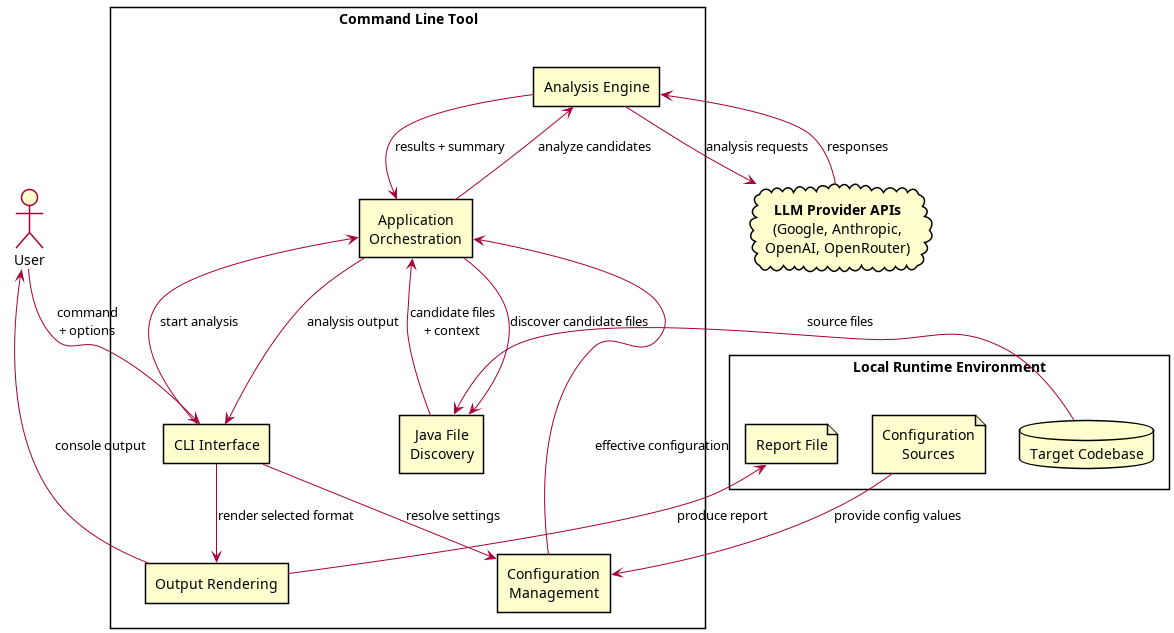
\includegraphics[width=\textwidth]{figures/component_diagram.png}
    \caption{Components of the SQL antipattern detection tool.}
    \label{fig:toolComponents}
\end{figure}

\section{Workflow}\label{sec:workflow}

Although the tool is implemented as a monolithic application, its internal architecture is organised as the staged pipeline shown in Figure~\ref{fig:toolWorkflow}. The main stages of the pipeline are the following:

\begin{itemize}
      \item \textbf{Input and configuration:} The tool receives command-line arguments, validates the input directory, and combines command-line options, environment variables, an optional configuration file, and built-in defaults into a single validated runtime configuration.
      \item \textbf{Model setup:} The selected model is resolved from an explicit provider-prefixed identifier. The provider prefix determines which LLM client is created and which API key is required.
      \item \textbf{Source-file discovery:} The selected project directory is recursively scanned for Java source files. The tool then applies jOOQ-oriented inclusion and exclusion heuristics to retain only files likely to contain relevant schema or query logic.
      \item \textbf{Candidate preparation:} Each retained Java file is converted into an analysis candidate containing its path, contents, analysis category, and optional contextual information. The analysis category determines whether the file is analysed as schema-definition code or query/application code. The tool also attaches the closest available key-definition context when such context is found.
      \item \textbf{Per-file analysis:} Candidate files are processed concurrently up to the configured concurrency limit. For each candidate, the source code is converted into a line-numbered representation and inserted into an LLM request. When the prompt-size budget requires it, the source context and any attached key-definition context are truncated while preserving useful context where possible.
      \item \textbf{Validation and failure handling:} If a request fails or returns data in an unexpected format, the tool retries it according to the configured retry count. If all attempts fail, the error is reported as a per-file result instead of aborting the whole run.
      \item \textbf{Aggregation and rendering:} After all candidates have been processed, the tool sorts the per-file results, computes a run-level summary, and renders the structured result as text, JSON, or CSV. The rendered output is then written either to standard output or to a configured output file.
\end{itemize}

\begin{figure}[H]
    \centering
    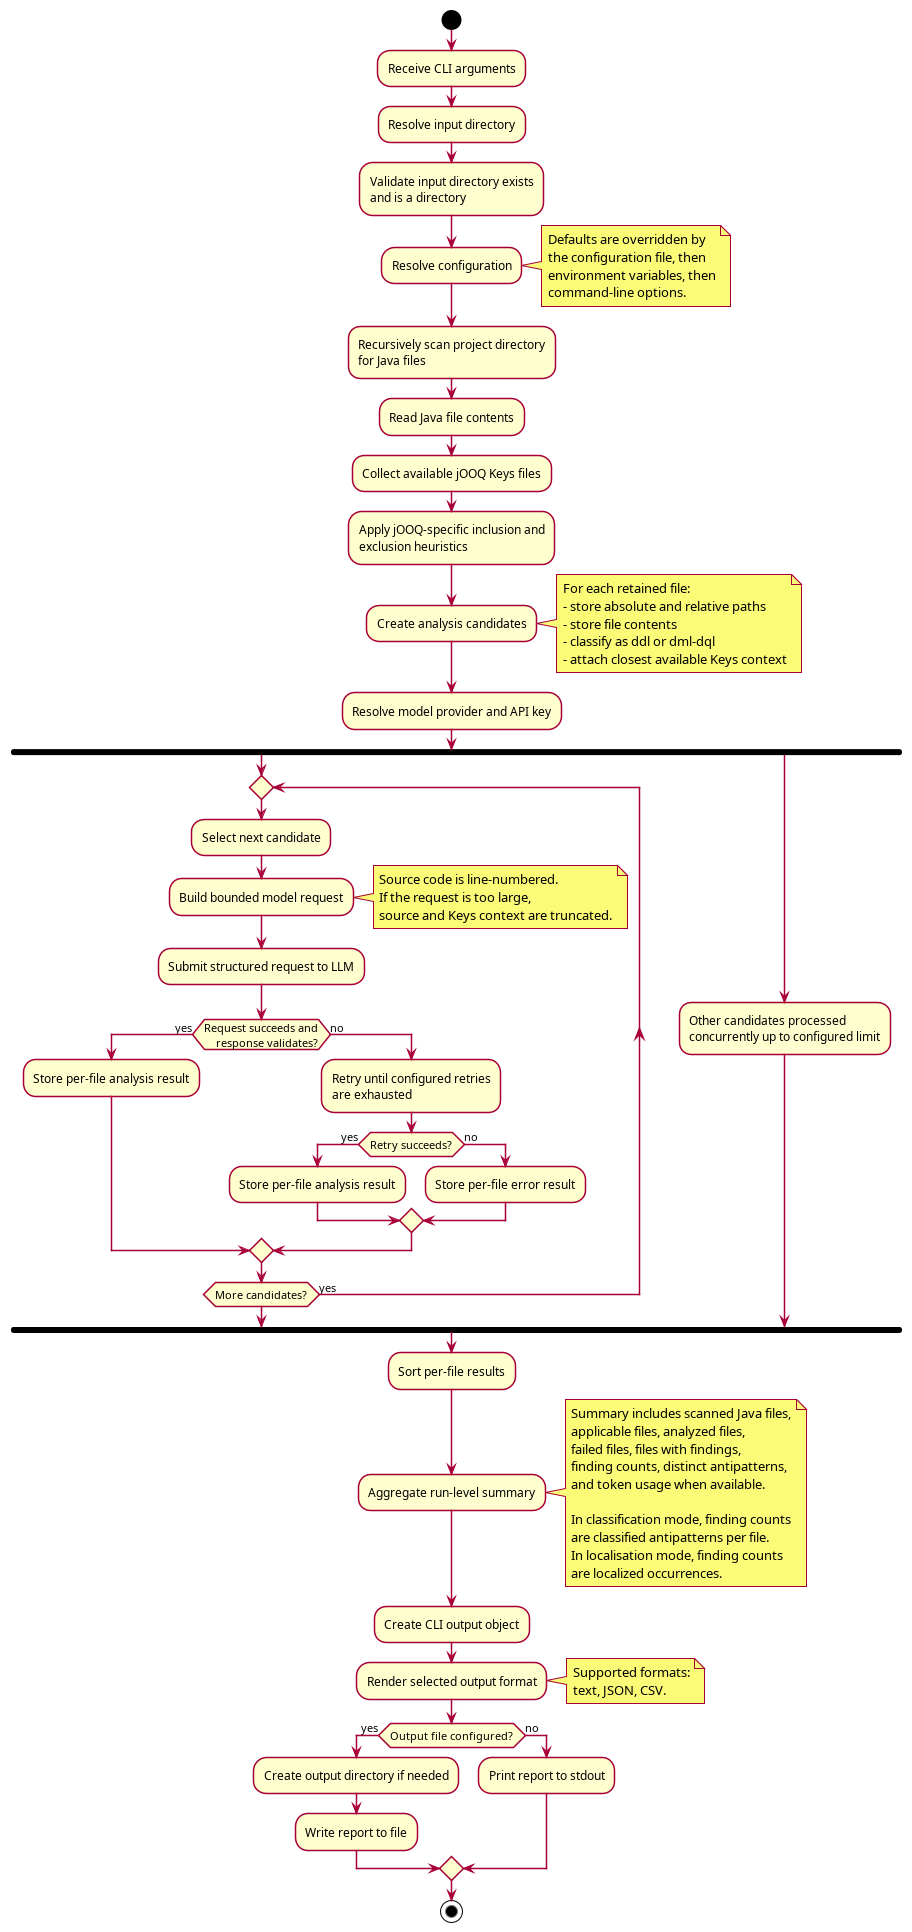
\includegraphics[width=320pt]{figures/tool_workflow.png}
    \caption{Workflow of the SQL antipattern detection tool.}
    \label{fig:toolWorkflow}
\end{figure}

\section{Result Representation}

The tool supports two analysis modes. In localisation mode, the output contains occurrence-level findings with source locations and explanations. In classification mode, the output contains only the distinct antipatterns detected in each file. The output of a run is a structured report consisting of run-level metadata, aggregate statistics, and per-file analysis results. The text rendering is intended for human inspection, while JSON and CSV outputs support automated processing, evaluation scripts, and integration with other tools.

Figure~\ref{fig:toolResults} shows a shortened text rendering of an analysis report in the localisation mode. The report begins with the selected model and analysed directory, followed by aggregate statistics. Individual findings are then grouped by file and include the detected antipattern, source location, relevant code fragment, and an explanation.

\bigskip % Add space before the figure
\begingroup % Start a local scope
\captionsetup{type=figure}
\phantomsection
\captionlistentry[figure]{Results displayed by the tool (truncated).}\label{fig:toolResults}
\begin{lstlisting}[
    frame=none, 
    basicstyle=\small, 
    breaklines=true, 
    breakatwhitespace=false, 
    breakindent=0pt,
    emph={jOOQ, Antipattern, Detector, Summary, Findings, Implicit, Columns, ID, Required},
    emphstyle=\bfseries,
    literate={!!!}{}{0} 
]
jOOQ Antipattern Detector
Model      google:gemini-3.1-flash-lite-preview
Directory  /home/kristo/masters-thesis/sample-project

Summary
Scanned Java files       164
Applicable files          39
Analyzed files            39
Failed files               0
Files with findings        7
Total occurrences         14
Distinct antipatterns      2
Input tokens           68739
Output tokens           1925
Total tokens           70664

Findings
  ----------------------------------------
src/main/java/com/inventory/prosta/bot/jooq/tables/AccountChat.java
  ID Required (54-54)
  Code        public final TableField<AccountChatRecord, Long> I!!!D = createField(DSL.name("id"), SQLDataType.BIGINT.nullable(false).identity(true), this, "");
  Explanation The primary key is named 'id', which is a generic name that provides no semantic information about the entity. Consider renaming it to 'account_chat_id' to improve clarity and consistency across the database schema.
  ----------------------------------------
src/main/java/com/inventory/prosta/bot/repository/AccountRepo.java
  Implicit Columns (64-64)
  Code        dsl.select()
  Explanation Using select() without arguments fetches all columns from the table, which can lead to performance issues and unnecessary data transfer. Explicitly list only the required columns in the select clause.

  Implicit Columns (90-90)
  Code        dsl.select(ACCOUNT.fields())
  Explanation Using ACCOUNT.fields() fetches all columns from the table, which is inefficient if only a subset of data is needed. Specify only the necessary columns to improve query performance and maintainability.
\end{lstlisting}

\nopagebreak
\begin{minipage}{\linewidth}
    \captionof*{figure}{Figure \thefigure. Results displayed by the tool (truncated).}
\end{minipage}
\par % Apply the paragraph settings *inside* the group
\endgroup % Revert to global normalsize and paragraph spacing
\bigskip % Add space after the figure

\section{Implementation Technologies}

The tool utilises the following technologies:

\begin{itemize}
    \item \textbf{Bun \nobreakcite{bunHomepage}:} Modern JavaScript toolkit, consisting of a JavaScript runtime, bundler, test runner, and package manager. It was selected for its high performance, simple setup, built-in support for TypeScript, and built-in ability to compile applications into standalone executables.
    \item \textbf{TypeScript \nobreakcite{typeScriptHomepage}:} Strongly typed superset of JavaScript, enabling developers to catch errors (e.g., type mismatches and nullability errors) during development, rather than at runtime. It was selected for its compile-time type safety and enhanced IDE support compared to JavaScript.
    \item \textbf{Biome \nobreakcite{biomeHomepage}:} Modern code formatter and linter for JavaScript and TypeScript. It was selected for its high performance, simple setup, and built-in support for TypeScript.
    \item \textbf{Vercel AI SDK \nobreakcite{aiSdkHomepage}:} Standardised interface for communicating with LLM providers, hiding provider-specific interface differences behind a unified abstraction.
    \item \textbf{Commander \nobreakcite{commanderGitHub}:} Lightweight framework for building CLI applications, used for parsing command-line arguments.
    \item \textbf{fast-glob \nobreakcite{fastGlobGitHub}:} Performance-oriented library for traversing the file system and retrieving file paths based on “glob” patterns (e.g., \texttt{**/*.java}). Used to find relevant files in the directory of the analysed project.
    \item \textbf{p-limit \nobreakcite{pLimitGitHub}:} Library for running multiple asynchronous functions with limited concurrency. Used to perform a limited number of parallel requests against the LLM provider.
    \item \textbf{Zod \nobreakcite{zodHomepage}:} TypeScript-first library for schema validation. Used for defining schemas for configuration options and LLM responses, and for validating objects against their respective schemas.
\end{itemize}

\section{Configuration Interface}\label{sec:configurationOptions}

The configuration interface was designed to support both interactive use and automated evaluation runs. The available options can be grouped into five categories: model selection, analysis behaviour, execution control, output control, and provider authentication. This made it possible to reuse the same implementation for manual inspection, quantitative experiments, and automated result collection.

Although the tool provides user-friendly defaults for common command-line usage, most of the execution parameters can be overridden to support controlled experiments. For example, the output format can be changed from human-readable text to JSON or CSV, allowing results to be consumed by evaluation scripts or third-party tooling. Similarly, while the default prompts are embedded within the executable binary to keep the tool fully self-contained by default, they can be loaded from a JSON file with an execution parameter, enabling the use of other prompting strategies or the detection of additional antipatterns.

A comprehensive overview of all available configuration options, including their accepted parameters and default values, is provided in Appendix~\ref{chapter:appendix-configuration-options}.

\section{Quantitative Analysis}\label{sec:developmentQuantitative}

To validate the detection performance of the finalised tool, we performed an analysis on each project in the test set produced in Section~\ref{sec:dataSplit}, using the tool in the default “localisation” mode. As in Section~\ref{sec:experimentsQuantitative}, we evaluated the tool using metrics suitable for a multi-label multi-occurrence localisation task: IoU and F1-score.

So far, we have treated the task as a localisation task, and validating it as such; however, there is not much comparison data available for such an approach. To compare our results against other works regarding detecting antipatterns and code smells using LLMs, we also evaluated it as a multi-label classification task.

To achieve this, we re-analysed the projects in the test set, this time using the tool in the “classification” mode, and compared the results against the ground truth. In this case, a prediction was considered a TP, if the tool detected an antipattern within a file, and the ground truth also contained the same antipattern within that file.

Based on the results of the quantitative analysis, we provide an answer to \textbf{RQ3} in Section~\ref{sec:resultsRQ3}. We compare our performance metrics against previous works regarding both SQL antipattern detection and LLM-based code smell detection in Section~\ref{sec:comparison}.

\section{Qualitative Analysis}

We manually inspected the differences between the tool's results and the ground truth, seeking patterns within the FPs and FNs and discussing their root causes in Section~\ref{sec:detectionErrors}.

We also compared the outputs of the “localisation” and “classification” modes. The differences in the results were analysed to identify common localisation errors and their underlying causes, and to explain why classification metrics may yield stronger results than localisation metrics.